\documentclass{beamer}
\usetheme{default}

\usepackage{amsmath}
\usepackage{amsthm}
\usepackage{amssymb}
\usepackage{mathtools}
\usepackage{xcolor}
\usepackage{hyperref}
\hypersetup{
  colorlinks=true,
  linkcolor=blue,
  urlcolor=blue
}
\usepackage{cleveref}

\usepackage{siunitx}

\title{Speech Digit Recognition}
\author{Blake Freer}
\date{April 2025}

\begin{document}
\frame{\titlepage}

\begin{frame}
  \frametitle{Free Spoken Digit Dataset}
  \vfill
  \begin{itemize}
    \item 6 different speakers
    \item 3000 .wav files (50 per digit per speaker)
    \item Pre-segmented to digit
    \item \qty{8}{\kilo\hertz} sample rate
  \end{itemize}
  \vfill
  \tiny\url{https://github.com/Jakobovski/free-spoken-digit-dataset}
\end{frame}

\begin{frame}
  \frametitle{Pipeline}
  \begin{figure}[h]
    \centering
    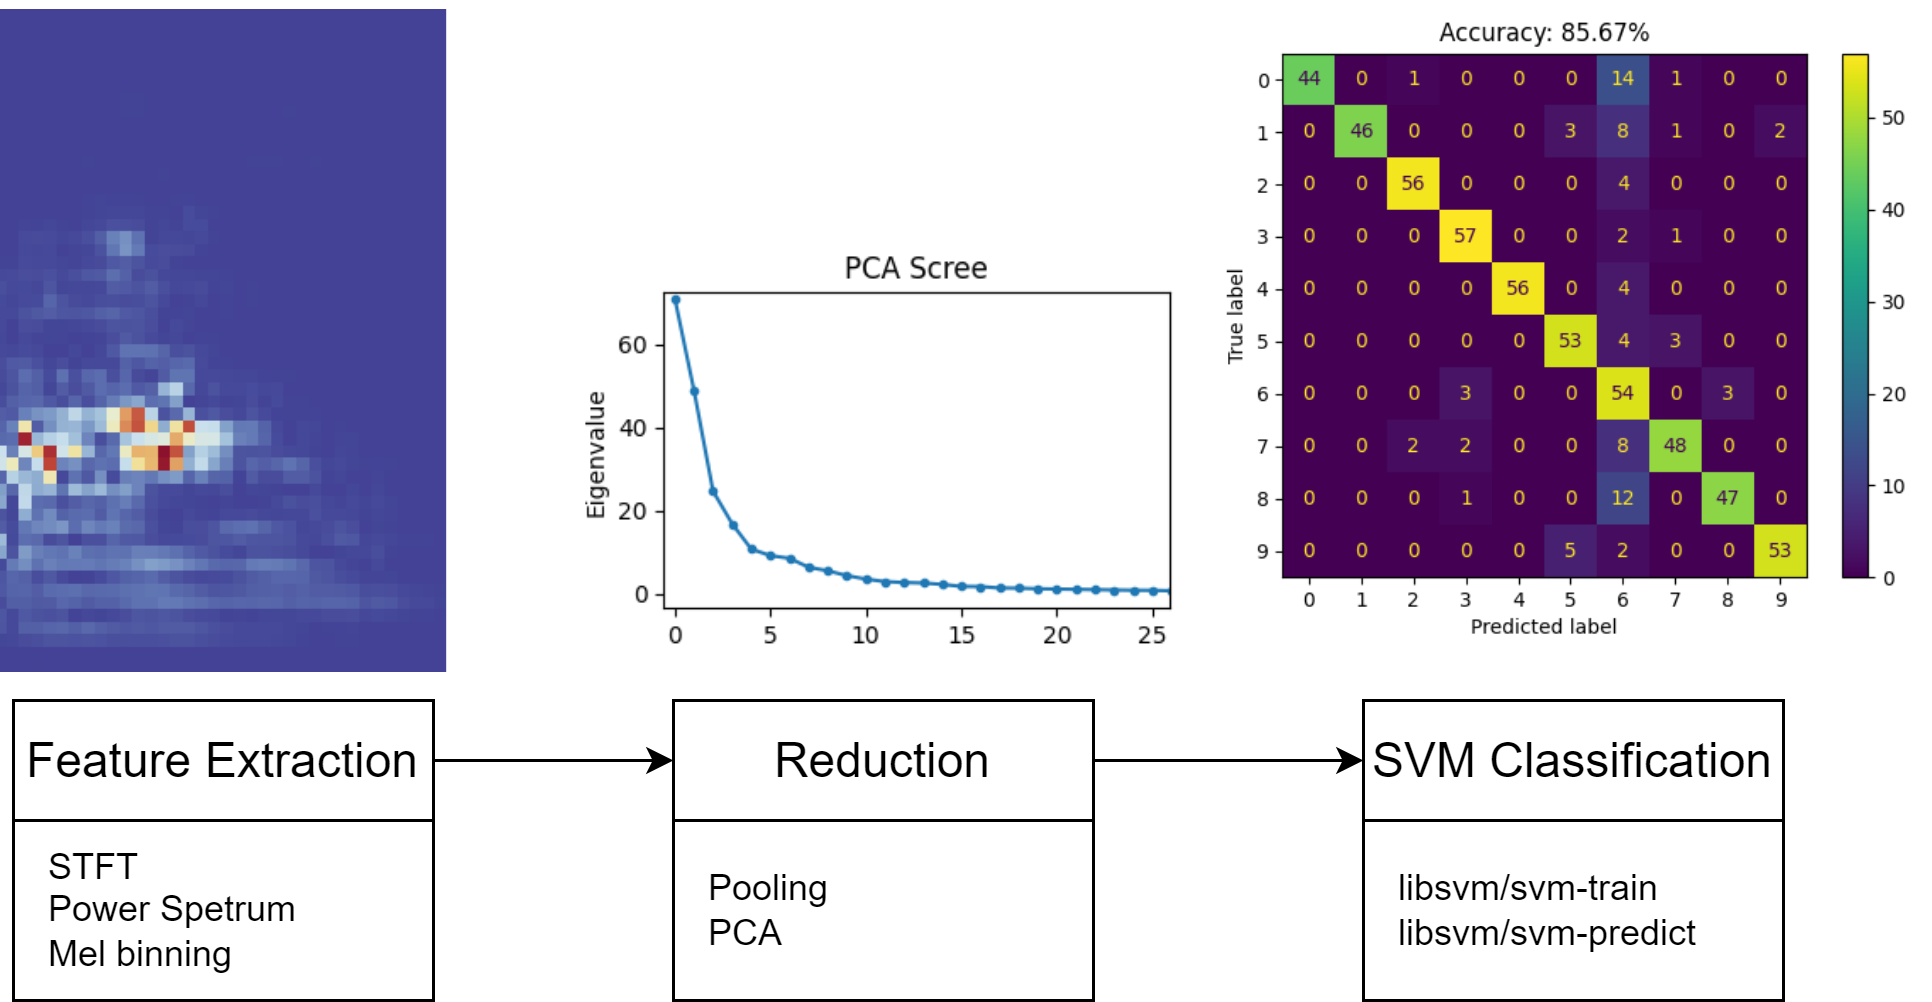
\includegraphics[width=\textwidth]{img/pipeline-pipeline.png}
  \end{figure}
\end{frame}

\begin{frame}
  \frametitle{Feature Extraction}
  \begin{figure}[h]
    \centering
    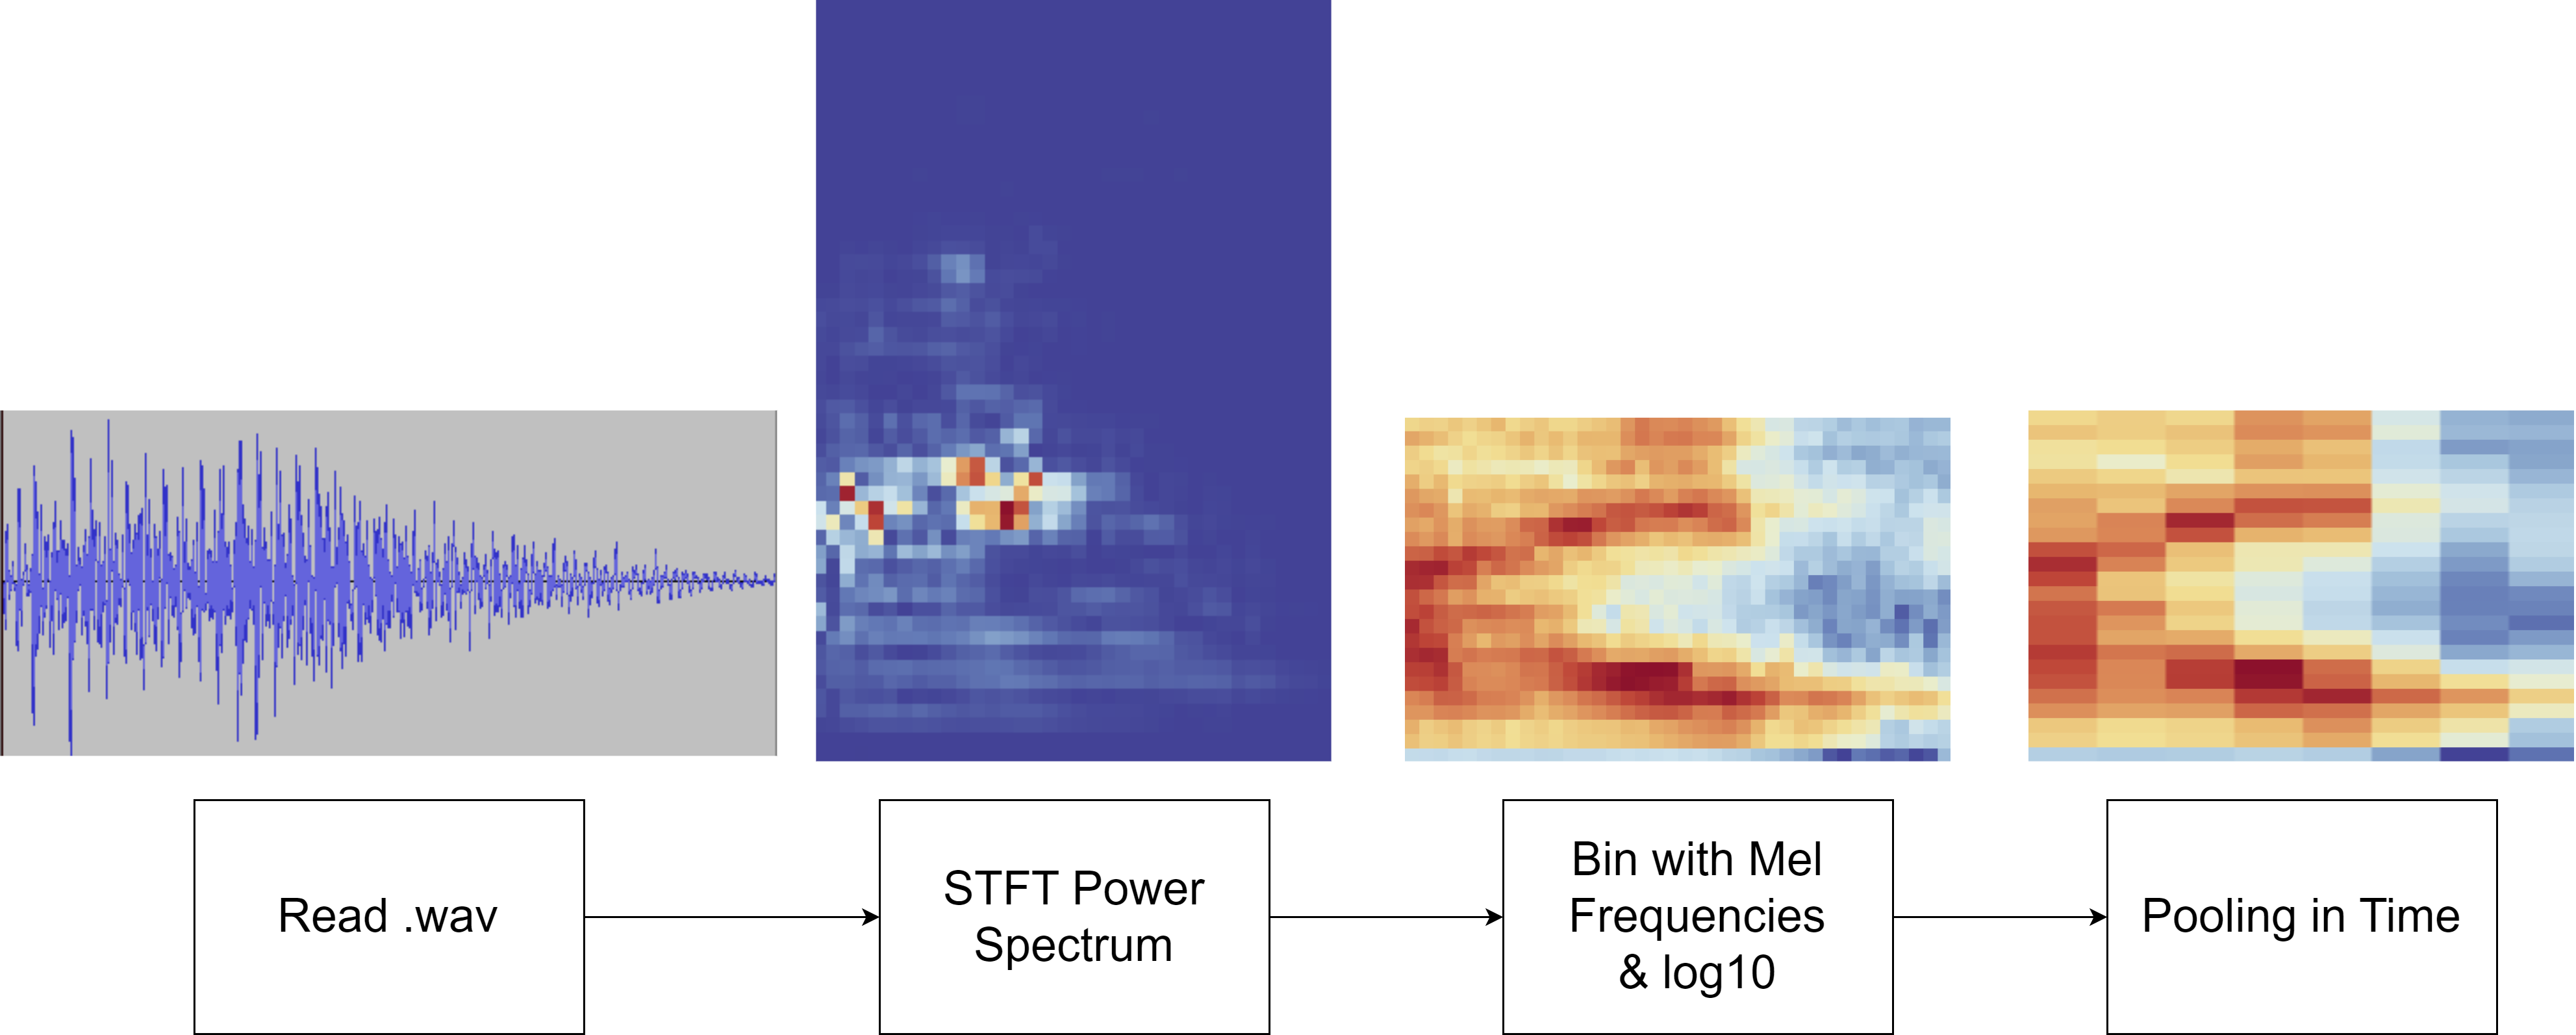
\includegraphics[width=\textwidth]{img/pipeline-feature.png}
  \end{figure}
\end{frame}

\end{document}
